\documentclass[10pt,oneside]{article}

\usepackage[T1]{fontenc}
\usepackage{fontawesome}

\usepackage[paper=a4paper,margin=2cm,bottom=2.5cm]{geometry}
\usepackage[sfdefault,light,condensed]{roboto}
\usepackage[export]{adjustbox}
\usepackage[usenames,dvipsnames,table]{xcolor}

\usepackage{amsmath,amssymb,array,fancyhdr,graphicx,enumitem,lastpage,multicol,tabularx,textcomp,titlesec}
\usepackage{mathtools}

\setlength\extrarowheight{1pt}
\setlength\parindent{0cm}
\renewcommand\headrule{}
\setlength{\footskip}{1.25cm}

\pagestyle{fancy}

\definecolor{BoxHeaderBG}{RGB}{50, 50, 50}
\definecolor{BoxHeaderText}{RGB}{255, 255, 255}

\newcommand{\BoxHeader}[2]{
    \multicolumn{#1}{| >{\bfseries\footnotesize\cellcolor{BoxHeaderBG}\arraybackslash}l |}{
        \textcolor{BoxHeaderText}{#2}
    }
}

\definecolor{ATLHeaderBG}{RGB}{65, 190, 30}
\definecolor{ATLHeaderText}{RGB}{0, 0, 0}

\definecolor{ATLSkillBG}{RGB}{215, 230, 210}
\definecolor{ATLSkillText}{RGB}{0, 0, 0}

\definecolor{DefinitionBoxHeaderBG}{RGB}{30, 30, 110}
\definecolor{DefinitionBoxHeaderText}{RGB}{255, 255, 255}

\definecolor{FormativeHeaderBG}{RGB}{150, 30, 150}
\definecolor{FormativeHeaderText}{RGB}{255, 255, 255}

\definecolor{GlobalContextHeaderBG}{RGB}{255, 255, 150}
\definecolor{GlobalContextHeaderText}{RGB}{0, 0, 0}

\definecolor{KeyConceptHeaderBG}{RGB}{15, 225, 225}
\definecolor{KeyConceptHeaderText}{RGB}{0, 0, 0}

\definecolor{RelatedConceptHeaderBG}{RGB}{15, 170, 170}
\definecolor{RelatedConceptHeaderText}{RGB}{0, 0, 0}

\definecolor{QuestionHeaderBG}{RGB}{240, 240, 240}
\definecolor{QuestionHeaderText}{RGB}{0, 0, 0}

\definecolor{SolutionHeaderBG}{RGB}{225, 150, 110}
\definecolor{SolutionHeaderText}{RGB}{0, 0 , 0}

\definecolor{SummativeHeaderBG}{RGB}{195, 15, 15}
\definecolor{SummativeHeaderText}{RGB}{255, 255, 255}

\newcommand{\ATLHeader}[1]{
    \cellcolor{ATLHeaderBG}\textcolor{ATLHeaderText}{
        \bfseries\footnotesize
        ATL SKILL (#1) \hfill \faGears
    }
}

\newcommand{\ATLSkill}[1]{
    \cellcolor{ATLSkillBG}\textcolor{ATLSkillText}{
        \itshape #1
    }
}

\newcommand{\DefinitionBoxHeader}{
    \cellcolor{DefinitionBoxHeaderBG}\textcolor{DefinitionBoxHeaderText}{
        \bfseries\footnotesize
        DEFINITIONS \hfill \faPencil
    }
}

\newcommand{\FormativeHeader}{
    \cellcolor{FormativeHeaderBG}\textcolor{FormativeHeaderText}{
        \bfseries\footnotesize
        FORMATIVE ASSESSMENT \hfill \faComments
    }
}

\newcommand{\GlobalContextHeader}[1]{
    \cellcolor{GlobalContextHeaderBG}\textcolor{GlobalContextHeaderText}{
        \bfseries\footnotesize
        GLOBAL CONTEXT (#1) \hfill \faGlobe
    }
}

\newcommand{\KeyConceptHeader}[1]{
    \cellcolor{KeyConceptHeaderBG}\textcolor{KeyConceptHeaderText}{
        \bfseries\footnotesize
        KEY CONCEPT (#1) \hfill \faKey
    }
}

\newcommand{\RelatedConceptHeader}[1]{
    \cellcolor{RelatedConceptHeaderBG}\textcolor{RelatedConceptHeaderText}{
        \bfseries\footnotesize
        RELATED CONCEPT (#1) \hfill \faLink
    }
}

\newcommand{\SolutionHeader}[1]{
    \cellcolor{SolutionHeaderBG}\textcolor{SolutionHeaderText}{
        \bfseries\footnotesize 
        #1 \hfill \faPaste
    }
}

\newcommand{\SummativeHeader}{
    \cellcolor{SummativeHeaderBG}\textcolor{SummativeHeaderText}{
        \bfseries\footnotesize
        SUMMATIVE ASSESSMENT \hfill \faCheck
    }
}

\newcounter{QuestionCounter}

\newcommand{\QuestionBox}[1]{
    \stepcounter{QuestionCounter}
    \cellcolor{QuestionHeaderBG}\textcolor{QuestionHeaderText}{
        {\bfseries\scriptsize Q\theQuestionCounter} #1
    }
}

\newcommand{\boxwidth}{\linewidth}

\lhead{\scriptsize\texttt{U\UnitNumber: \UnitTitle \\ L\LessonNumber: \LessonTitle}}
\rhead{\scriptsize\ttfamily [DESIGN/\CourseName/U\UnitNumber/L\LessonNumber]\\\ }

\lfoot{
\includegraphics[height=2cm,valign=c]{Files/logo}}
\cfoot{\footnotesize DESIGN/\CourseName/U\UnitNumber/L\LessonNumber\ | \LessonTitle \\ Woodstock School | Mussoorie, Uttarakhand, India}
\rfoot{
\includegraphics[height=2cm,valign=c]{Files/ib-world-school-logo-1-colour}}

\titleformat{\section}{\normalfont\Large\bfseries}{}{0em}{}[{\titlerule[0.5pt]}]
\titleformat{\subsection}{\normalfont\large\bfseries}{}{0em}{}


\usepackage{circuitikz,subcaption,tikzsymbols}

\usetikzlibrary{arrows,calc,shapes.misc}

\tikzset{cross/.style={cross out, draw, 
         minimum size=2*(#1-\pgflinewidth), 
         inner sep=0pt, outer sep=0pt}}

\def\CourseName{MYP3}

\def\LessonNumber{03}
\def\LessonTitle{Series \& Parallel Circuits}

\def\UnitNumber{01}
\def\UnitTitle{Circuits \& Electronics}

\begin{document}
    \textbf{\large Name: } \rule{12cm}{0.5pt} \hfill \textbf{\large Section: } \rule{1cm}{0.5pt}

    \begin{center}
        \huge\bfseries
        \LessonTitle
    \end{center}

    \section{Before You Begin}
    \begin{tabularx}{\boxwidth}{| X |}
        \hline
        \GlobalContextHeader{Orientation in Space \& Time}\\\hline
        \QuestionBox{There are numerous cultures around the world, such as the famous American Amish, which shun the adoption of technology for various reasons. What do you think motivates these people to avoid embracing modern technology, espeically the use of electricity?}\\\hline
        \ \\[5cm]\hline
        \QuestionBox{There are also groups of people, such as the Sentinelese in the Bay of Bengal, who reject contact with the outside world. This means that they have never had significant exposure to the use of electricity. What do you think would happen to the culture of these people if they were to be exposed to and adopted modern technology?}\\\hline
        \ \\[5cm]\hline
    \end{tabularx}

    \smallskip
    \begin{tabularx}{\boxwidth}{| X |}
        \hline
        \RelatedConceptHeader{Invention}\\\hline
        \QuestionBox{Many of the great inventions in human history have revolved around the reduction of manual labour. Why do you think the reduction of \emph{work} for humans is a major motivation for the invention of new technology?}\\\hline
        \ \\[5cm]\hline
    \end{tabularx}

    \pagebreak
    \section{Technical Background}
    So far, all of the circuits we have built have revolved around a single ``loop'' of electric current. These simple circuits are called \emph{series circuits}.

    \medskip
    This lesson focuses on the difference between building a circuit in \emph{series} and \emph{parallel}, as defined below.

    \subsection{Series Circuits}

    \begin{minipage}{0.26\boxwidth}
        \centering
        \begin{circuitikz}
            \draw (0, 1) node[left,yshift=-5] {+} to [battery1] (0, 0);
            \node at (-0.75, 0.5) {3V};
            \draw (0, 1) |- (1, 2) to [full led] (2, 2) -- (3, 2) |- (2, -1) to [full led] (1, -1) -| (0, 0);
        \end{circuitikz}
    \end{minipage}
    \begin{minipage}{0.025\boxwidth}
        \ 

    \end{minipage}
    \begin{minipage}{0.35\boxwidth}
        In a simple series circuit such as the one given here, electrical energy passes through one component before entering the next.
    \end{minipage}
    \begin{minipage}{0.26\boxwidth}
        \centering
        \begin{circuitikz}
            \draw (0, 1) node[left,yshift=-5] {+} to [battery1] (0, 0);
            \node at (-0.75, 0.5) {3V};
            \draw (0, 1) |- (1, 2) to [full led] (2, 2) -- (3, 2) |- (2, -1) to [full led] (1, -1) -| (0, 0);

            \draw[->, >=triangle 45,very thick, red] (0.5, 0.75) |- (2.5, 1.5) |- (2.5, -0.5) -| (0.5, 0.5);
        \end{circuitikz}
    \end{minipage}

    \subsection{Parallel Circuits}
    \begin{minipage}{0.3\boxwidth}
        \centering
        \begin{circuitikz}
            \draw (0, 1) node[left,yshift=-5] {+} to [battery1] (0, 0);
            \node at (-0.75, 0.5) {3V};
            \draw (0, 1) |- (2, 2) -| (3, 1) to [full led] (3, 0);
            \draw (1.5, 2) -- (1.5, 1) to [full led] (1.5, 0);
            \draw (3, 0) -- (3, -1) -| (0, 0);
            \draw (1.5, 0) -- (1.5, -1);
        \end{circuitikz}
    \end{minipage}
    \begin{minipage}{0.34\boxwidth}
        In parallel circuits, electrical energy splits along multiple paths. This allows voltage to remain the same across all components, while dividing current.
    \end{minipage}
    \begin{minipage}{0.3\boxwidth}
        \centering
        \begin{circuitikz}
            \draw (0, 1) node[left,yshift=-5] {+} to [battery1] (0, 0);
            \node at (-0.75, 0.5) {3V};
            \draw (0, 1) |- (2, 2) -| (3, 1) to [full led] (3, 0);
            \draw (1.5, 2) -- (1.5, 1) to [full led] (1.5, 0);
            \draw (3, 0) -- (3, -1) -| (0, 0);
            \draw (1.5, 0) -- (1.5, -1);

            \draw[->, >=triangle 45,very thick, red] (0.5, 0.75) |- (1.4, 1.5) |- (1.25, -0.5) -- (0.5, -0.5) -- (0.5, 0.5);
            \draw[->, >=triangle 45,very thick, red] (0.5, 0.75) |- (2.5, 1.5) |- (2.5, -0.5) -- (0.5, -0.5) -- (0.5, 0.5);

            \draw[->,>=stealth,very thick, blue] (0.75, 1.4) -- (1.95, 1.4);
            \draw[->,>=stealth,very thick, blue] (1.05, 1.15) +(100:0.25) arc 
            (100:-20:0.25);
        \end{circuitikz}
    \end{minipage}

    \subsection{Resistors in Series}
    Because resistors are used to restrict the flow of electricity, or \emph{current}, they behave differenty in series circuits versus parallel circuits.

    \medskip
    In series circuits, the \emph{total resistance} in the circuit is calculated as the sum of each resistor.
    
    \subsubsection*{Example}
    \begin{minipage}{0.3\boxwidth}
        \begin{center}
            \begin{circuitikz}
                \draw (0, 1) node[left,yshift=-5] {+} to [battery1] (0, 0);
                \node at (-0.75, 0.5) {3V};
                \draw (0, 1) |- (1, 2) to [european resistor,label=$220\ \Omega$] (2, 2) -| (3, 1) to [european resistor,label=$1\ \text{k}\Omega$] (3, 0) |- (2, -1) to [european resistor,label=$330\ \Omega$] (1, -1) -| (0, 0);
            \end{circuitikz}
        \end{center}
    \end{minipage}
    \begin{minipage}{0.375\boxwidth}
        \[\begin{aligned}
            \text{R}_\text{total} &= \text{R}_1 + \text{R}_2 + \text{R}_3 \\
            &= 220 + 1000 + 330\\
            &= 1550\ \Omega
        \end{aligned}\]
    \end{minipage}

    \bigskip
    \begin{tabularx}{\boxwidth}{| X |}
        \hline
        \SolutionHeader{Calculating Total Resistance in a Series Circuit} \\\hline
        The above example yields the following formula:\\
        \hfill R$_{\text{total}} = \text{R}_{1} + \text{R}_{2} + \cdots + \text{R}_{n}$ \hfill\, \\
        This is a very simple formula, but can be applied in a variety of ways to create circuits with various target resistances.\\\hline
    \end{tabularx}

    \pagebreak
    \subsection{Resistors in Parallel}
    Because parallel circuits \emph{divide current}, it becomes a bit harder to determine total resistance in the type of circuits seen below.

    \subsubsection*{Example \#1}
    Rarely, all resistors in the circuit will have the same value as in this first example. In that case, all you need to do is divide the resistor value by the number of parallel paths in the circuit.

    \bigskip
    \begin{minipage}{0.45\boxwidth}
        \begin{circuitikz}
            \draw (0, 1) node[left,yshift=-5] {+} to [battery1] (0, 0);
            \node at (-0.75, 0.5) {3V};
            \draw (0, 1) |- (1.75, 2) -- (1.75, 1) to [european resistor,label=\small$330\ \Omega$] (1.75, 0) -- (1.75, -1) -| (0, 0);
            \draw (1, 2) -| (3.5, 1) to [european resistor,label=\small$330\ \Omega$] (3.5, 0) -- (3.5, -1) -| (0, 0);
            \draw (3.5, 2) -| (5.25, 1) to [european resistor,label=\small$330\ \Omega$] (5.25, 0) -- (5.25, -1) -| (0, 0);
        \end{circuitikz}
    \end{minipage}
    \begin{minipage}{0.2\boxwidth}
        \[\begin{aligned}
            \text{R}_{\text{total}} &= \frac{\text{R}}{3} \\[8pt]
            &= \dfrac{330}{3} \\[8pt]
            &= 110\ \Omega
        \end{aligned}\]
    \end{minipage}

    \subsubsection*{Example \#2}
    The result is less obvious for more complex parallel circuits. To understand what is going on, let's make a small chart of values for the current passing through each resistor. Remember: in a parallel circuit such as this one the voltage across all components remains the same. Keep in mind that \emph{Ohm's Law} gives us a formula for current: $I = \frac{V}{R}$.

    \bigskip
    \begin{minipage}{0.475\boxwidth}
        \begin{circuitikz}
            \draw (0, 1) node[left,yshift=-5] {+} to [battery1] (0, 0);
            \node at (-0.75, 0.5) {3V};
            \draw (0, 1) |- (1.75, 2) -- (1.75, 1) to [european resistor,label=\small$220\ \Omega$] (1.75, 0) -- (1.75, -1) -| (0, 0);
            \draw (1, 2) -| (3.5, 1) to [european resistor,label=\small$470\ \Omega$] (3.5, 0) -- (3.5, -1) -| (0, 0);
            \draw (3.5, 2) -| (5.25, 1) to [european resistor,label=\small$1\ \text{k}\Omega$] (5.25, 0) -- (5.25, -1) -| (0, 0);
        \end{circuitikz}
    \end{minipage}
    \begin{minipage}{0.5\boxwidth}
        \begin{center}
            \newcolumntype{C}{>{\centering\arraybackslash}X}
            \renewcommand\arraystretch{1.5}
            \begin{tabularx}{\boxwidth}{| c | C | C | C |}
                \hline
                \cellcolor{black!25} & \textbf{R$_1$} & \textbf{R$_2$} & \textbf{R$_3$}\\\hline
                \textbf{V} & 3 & 3 & 3\\\hline
                \textbf{R} & 220 & 470 & 1000\\\hline    
                \textbf{I} & $\frac{3}{220} \approx 0.0136$ & $\frac{3}{470} \approx 0.0064$ & $\frac{3}{1000} = 0.0030$ \\\hline
            \end{tabularx}
        \end{center}
    \end{minipage}

    \bigskip
    From the above table, we can see that the \emph{total current} in the circuit is approximately $0.023$ amps (23 mA). Once again using \emph{Ohm's Law} $\left(R = \frac{V}{I}\right)$ gives us a \emph{total resistance} of: $R = \frac{3}{0.023} \approx 130.435\ \Omega$.

    \bigskip
    \renewcommand\arraystretch{1}
    \begin{tabularx}{\boxwidth}{| X |}
        \hline
        \SolutionHeader{Calculating Total Resistance of a Parallel Circuit}\\\hline
        The above work can be summarized by the following formula:\\
        \hfill R$_{\text{total}} = \dfrac{1}{\dfrac{1}{\text{R}_1} + \dfrac{1}{\text{R}_2} + \cdots + \dfrac{1}{\text{R}_n}}$ \hfill\, \\
        Although it looks complicated, the end result of this formula is identical to making a chart of values similar to what we did previously.\\\hline
    \end{tabularx}
   
    \bigskip
    \begin{tabularx}{\boxwidth}{| X | }
        \hline
        \ATLHeader{Communication Skills} \\\hline
        \ATLSkill{...use and interpret a range of discipline-specific terms and symbols...} \\\hline
        \QuestionBox{Apply the formula above to calculate the total resistance of a parallel circuit using the given resistor values ($220\ \Omega$, $470\ \Omega$, and $1000\ \Omega$).} \\\hline
        \ \\[1.75cm]\hline
        \ATLSkill{...make inferences and draw conclusions...}\\\hline
        \QuestionBox{Explain why using the formula did \emph{not} yield the exact same value as in our example.}\\\hline
        \ \\[1.75cm]\hline
    \end{tabularx}
   
    \pagebreak

    \section{Developing Technical Skills}

    \subsubsection*{Circuit \#7: Building a Parallel Circuit}
    This circuit emulates the simple example of a parallel circuit given in the technical background.

    \subsubsection*{You Will Need}
    \begin{itemize}[noitemsep]
        \item[(1)] CR2032 Battery
        \item[(2)] LEDs
        \item[(1)] Roll of Copper Tape
        \item[(1)] Roll of Cellophane Tape   
    \end{itemize}

    \subsubsection*{Directions}
    Create the following paper circuit, ignoring the different arrows for now. Those arrows will be used in the next activity.

    \begin{center}
        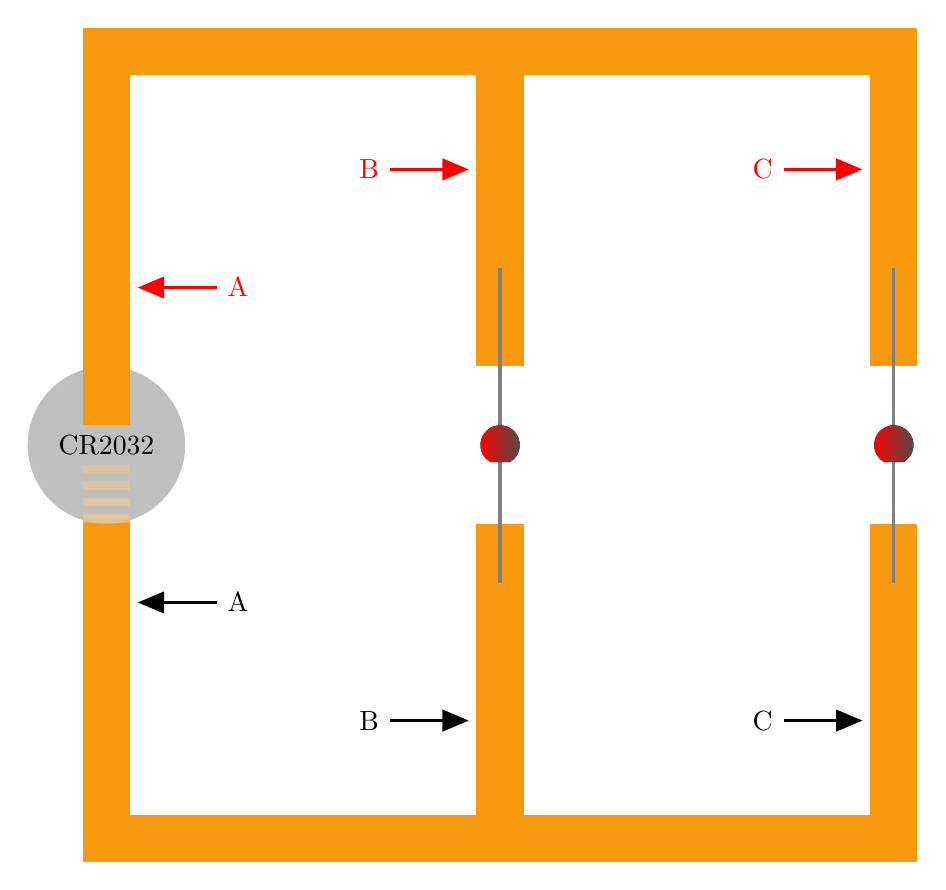
\begin{tikzpicture}
            \draw[line width=6mm,YellowOrange] (0, 0) -- (0, 5) -- (10, 5) -- (10, 1);
            \draw[line width=6mm,YellowOrange] (10, -1) -- (10, -5) -- (0, -5) -- (0, 0);

            \draw[line width=6mm,YellowOrange] (5, 5) -- (5, 1);
            \draw[line width=6mm,YellowOrange] (5, -1) -- (5, -5);

            \fill[black!25] (0, 0) circle (10mm);            
            \draw[line width=6mm, dashed,YellowOrange!50,draw opacity=0.5] (0, -0.25) -- (0, -1);
            \draw[line width=6mm,YellowOrange] (0, 0.25) -- (0, 1);
            \node[align=center] at (0, 0) {CR2032};

            \draw[very thick,black!50] (5, 2.25) -- (5, -1.75);
            \fill[left color=red, right color=black!70] ([shift=(-60:2.5mm)]5,0) arc (-60:240:2.5mm);

            \draw[very thick,black!50] (10, 2.25) -- (10, -1.75);
            \fill[left color=red, right color=black!70] ([shift=(-60:2.5mm)]10,0) arc (-60:240:2.5mm);

            \draw[->,>=triangle 45,very thick,red] (1.4, 2) node[right] {A} -- (0.4, 2);
            \draw[->,>=triangle 45,very thick,black] (1.4, -2) node[right] {A} -- (0.4, -2);

            \draw[->,>=triangle 45,very thick,red] (3.6, 3.5) node[left] {B} --(4.6, 3.5);
            \draw[->,>=triangle 45,very thick,black] (3.6, -3.5) node[left] {B} -- (4.6, -3.5);

            \draw[->,>=triangle 45,very thick,red] (8.6, 3.5) node[left] {C} --(9.6, 3.5);
            \draw[->,>=triangle 45,very thick,black] (8.6, -3.5) node[left] {C} -- (9.6, -3.5);            
        \end{tikzpicture}
    \end{center}

    \bigskip\bigskip
    \begin{tabularx}{\boxwidth}{| X | }
        \hline
        \ATLHeader{Communication Skills} \\\hline
        \ATLSkill{...make inferences and draw conclusions...} \\\hline
        \QuestionBox{Why does placing the LEDs in parallel allow them to both light compared to the series circuit for two LEDs you created in Lesson \#1?} \\\hline
        \ \\[4cm]\hline
    \end{tabularx}

    % use of multimeter
    \subsubsection*{Using a Multimeter}
    A \emph{multimeter} is a special device that allows you to take different measurements, such as voltage, resistance, and current, in a circuit. A few examples of multimeters are shown below.

    % images of multimeters
    \begin{figure}[h]
        \centering
        \begin{subfigure}{0.25\boxwidth}
            \centering
            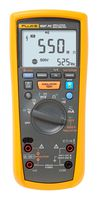
\includegraphics[height=4cm]{Extras/multimeter1}
        \end{subfigure}
        \begin{subfigure}{0.25\boxwidth}
            \centering
            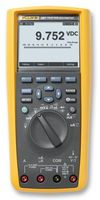
\includegraphics[height=4cm]{Extras/multimeter2}
        \end{subfigure}
        \begin{subfigure}{0.25\boxwidth}
            \centering
            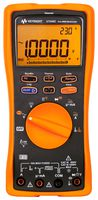
\includegraphics[height=4cm]{Extras/multimeter3}
        \end{subfigure}
        \caption*{\scriptsize Images courtesy element14.com.}
    \end{figure}


    While the complexity and capabilities of multimeters varies greatly, any multimeter available on the market today should be able to measure anything you'll need for this course. In particular, your multimeter should measure: DC Voltage, Resistance, Current (<10A).

    \medskip
    Because operating a multimeter can be highly dependent on the individual device, allow your teacher to demonstrate the use of the multimeter you have available to you before answering the following questions.

    \bigskip
    \begin{tabularx}{\boxwidth}{| X |}
        \hline
        \QuestionBox{Complete the following table of values by placing the appropriate probes at each labeled location in Circuit \#7.}\\\hline
    \end{tabularx}

    \begin{center}
        \newcolumntype{C}{>{\centering\arraybackslash}X}
        \begin{tabularx}{0.5\boxwidth}{| >{\bfseries\centering\arraybackslash}p{0.2cm} | C | C | C |}
            \hline
            \cellcolor{black!25} & \textbf{A} & \textbf{B} & \textbf{C} \\\hline
            \raisebox{-0.5cm}{V} & & & \\[1cm]\hline
            \raisebox{-0.5cm}{R} & & & \\[1cm]\hline
            \raisebox{-0.5cm}{I} & & & \\[1cm]\hline
        \end{tabularx}
    \end{center}

    \begin{tabularx}{\boxwidth}{| X |}
        \hline
        \ATLHeader{Communication Skills}\\\hline
        \ATLSkill{...make inferences and draw conclusions...}\\\hline
        \QuestionBox{Do the values match your expectations for a parallel circuit? Explain why or why not.}\\\hline
        \ \\[6cm]\hline
    \end{tabularx}


    \pagebreak
    % series resistors + multimeter
    \subsubsection*{Circuit \#8: Resistors in Series}
    The circuit below will allow you to explore the interaction between voltage, resistance, and current in a series circuit similar to the one shown in the technical background section.

    \subsubsection*{You Will Need}
    \begin{itemize}[noitemsep]
        \item[(1)] CR2032 Battery
        \item[(3)] Resistors ($220\ \Omega$, $330\ \Omega$, $470\ \Omega$)
        \item[(1)] Roll of Copper Tape
        \item[(1)] Roll of Cellophane Tape   
    \end{itemize}
    
    \subsubsection*{Directions}
    Create the following paper circuit. Then, complete the chart of voltage, resistance, and current using the multimeter at the indicated points.

    \bigskip
    \begin{minipage}[t]{0.7\boxwidth}\vspace*{0pt}
        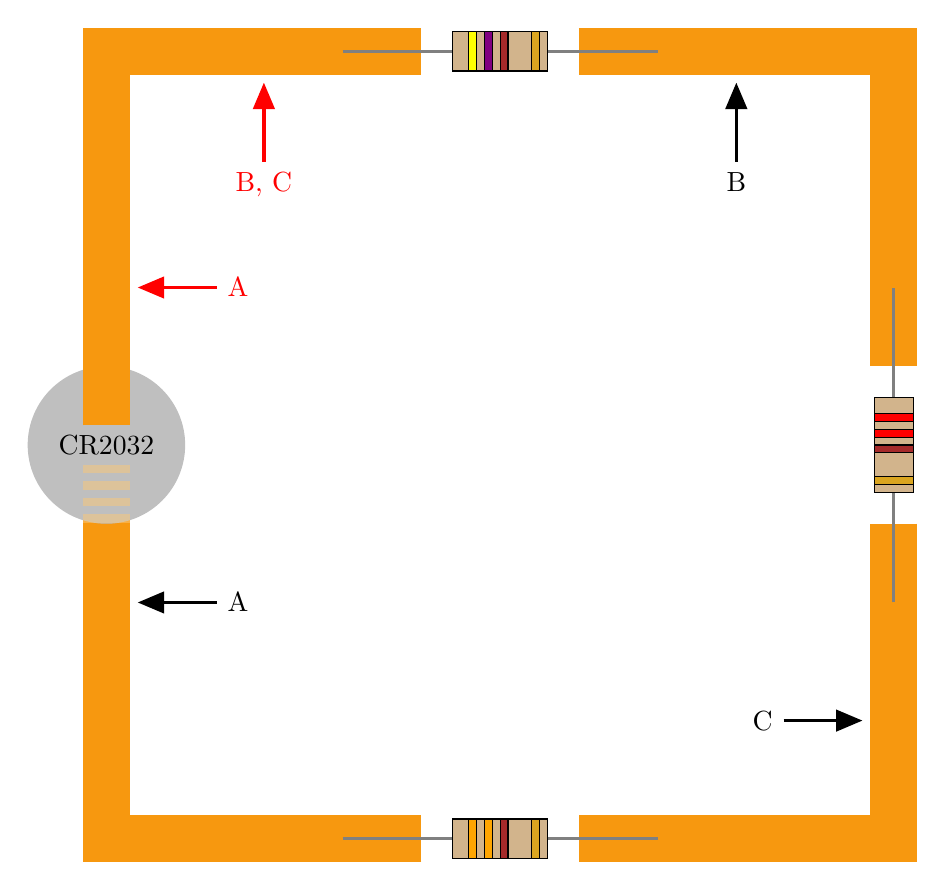
\begin{tikzpicture}
            \draw[line width=6mm,YellowOrange] (0, 0) |- (4, 5);
            \draw[line width=6mm,YellowOrange] (6, 5) -| (10, 1);
            \draw[line width=6mm,YellowOrange] (10, -1) |- (6, -5);
            \draw[line width=6mm,YellowOrange] (4, -5) -- (0, -5) -- (0, 0);

            \fill[black!25] (0, 0) circle (10mm);            
            \draw[line width=6mm, dashed,YellowOrange!50,draw opacity=0.5] (0, -0.25) -- (0, -1);
            \draw[line width=6mm,YellowOrange] (0, 0.25) -- (0, 1);
            \node[align=center] at (0, 0) {CR2032};
            
            \draw[->,>=triangle 45,very thick,red] (1.4, 2) node[right] {A} -- (0.4, 2);
            \draw[->,>=triangle 45,very thick,black] (1.4, -2) node[right] {A} -- (0.4, -2);
            
            \draw[->,>=triangle 45,very thick,red] (2, 3.6) node[below] {B, C} -- (2, 4.6);
            \draw[->,>=triangle 45,very thick,black] (8, 3.6) node[below] {B} -- (8, 4.6);

            \draw[->,>=triangle 45,very thick,black] (8.6, -3.5) node[left] {C} -- (9.6, -3.5);

            \coordinate (R1) at (10, -2);
            %220 Ohms
            \draw[very thick, black!50] (R1) -- ($(R1) + (0, 4)$);
            \draw[fill=Tan] ($(R1) + (0.25, 1.4)$) rectangle ($(R1) + (-0.25, 2.6)$);
            \draw[fill=Red] ($(R1) + (0.25, 2.4)$) rectangle ($(R1) + (-0.25, 2.3)$);
            \draw[fill=Red] ($(R1) + (0.25, 2.2)$) rectangle ($(R1) + (-0.25, 2.1)$);
            \draw[fill=Brown] ($(R1) + (0.25, 2.0)$) rectangle ($(R1) + (-0.25, 1.9)$);
            \draw[fill=Goldenrod] ($(R1) + (0.25, 1.6)$) rectangle ($(R1) + (-0.25, 1.5)$);

            \coordinate (R1) at (3, 5);
            %470 Ohms
            \draw[very thick, black!50] (R1) -- ($(R1) + (4, 0)$);
            \draw[fill=Tan ] ($(R1) + (1.4, 0.25)$) rectangle ($(R1) + (2.6, -0.25)$);
            \draw[fill=Yellow] ($(R1) + (1.6, 0.25)$) rectangle ($(R1) + (1.7, -0.25)$);
            \draw[fill=Purple] ($(R1) + (1.8, 0.25)$) rectangle ($(R1) + (1.9, -0.25)$);
            \draw[fill=Brown] ($(R1) + (2.0, 0.25)$) rectangle ($(R1) + (2.1, -0.25)$);
            \draw[fill=Goldenrod] ($(R1) + (2.5, 0.25)$) rectangle ($(R1) + (2.4, -0.25)$);

            \coordinate (R1) at (3, -5);
            %330 Ohms
            \draw[very thick, black!50] (R1) -- ($(R1) + (4, 0)$);
            \draw[fill=Tan ] ($(R1) + (1.4, 0.25)$) rectangle ($(R1) + (2.6, -0.25)$);
            \draw[fill=Orange] ($(R1) + (1.6, 0.25)$) rectangle ($(R1) + (1.7, -0.25)$);
            \draw[fill=Orange] ($(R1) + (1.8, 0.25)$) rectangle ($(R1) + (1.9, -0.25)$);
            \draw[fill=Brown] ($(R1) + (2.0, 0.25)$) rectangle ($(R1) + (2.1, -0.25)$);
            \draw[fill=Goldenrod] ($(R1) + (2.5, 0.25)$) rectangle ($(R1) + (2.4, -0.25)$);

        \end{tikzpicture}
    \end{minipage}
    \begin{minipage}{0.025\boxwidth}\vspace*{0pt}
        \

    \end{minipage} 
    \begin{minipage}[t]{0.25\boxwidth}\vspace*{0pt}
        \newcolumntype{C}{>{\centering\arraybackslash}X}
        \begin{tabularx}{\boxwidth}{| >{\bfseries\centering\arraybackslash}p{0.2cm} | C | C | C |}
            \hline
            \cellcolor{black!25} & \textbf{A} & \textbf{B} & \textbf{C} \\\hline
            \raisebox{-0.5cm}{V} & & & \\[1cm]\hline
            \raisebox{-0.5cm}{R} & & & \\[1cm]\hline
            \raisebox{-0.5cm}{I} & & & \\[1cm]\hline
        \end{tabularx}
    \end{minipage}
    
    \vspace{1cm}

    \begin{tabularx}{\boxwidth}{| X |}
        \hline
        \ATLHeader{Communication Skills}\\\hline
        \ATLSkill{...make inferences and draw conclusions...}\\\hline
        \QuestionBox{Are your measurements for \emph{current} what you expected based on where measurements were taken? Explain why the current behaves like this in a series circuit.}\\\hline
        \ \\[4cm]\hline
    \end{tabularx}

    % parallel circuit for resistors + multimeter
    \subsubsection*{Circuit \#9: Resistors in Parallel}
    The circuit below will allow you to explore the interaction between voltage, resistance, and current in a parallel circuit similar to the one shown in the technical background section.

    \subsubsection*{You Will Need}
    \begin{itemize}[noitemsep]
        \item[(1)] CR2032 Battery
        \item[(3)] Resistors ($220\ \Omega$, $330\ \Omega$, $1\ \text{k}\Omega$)
        \item[(1)] Roll of Copper Tape
        \item[(1)] Roll of Cellophane Tape   
    \end{itemize}
    
    \subsubsection*{Directions}
    Create the following paper circuit. Then, complete the chart of voltage, resistance, and current using the multimeter at the indicated points.

    \begin{center}
        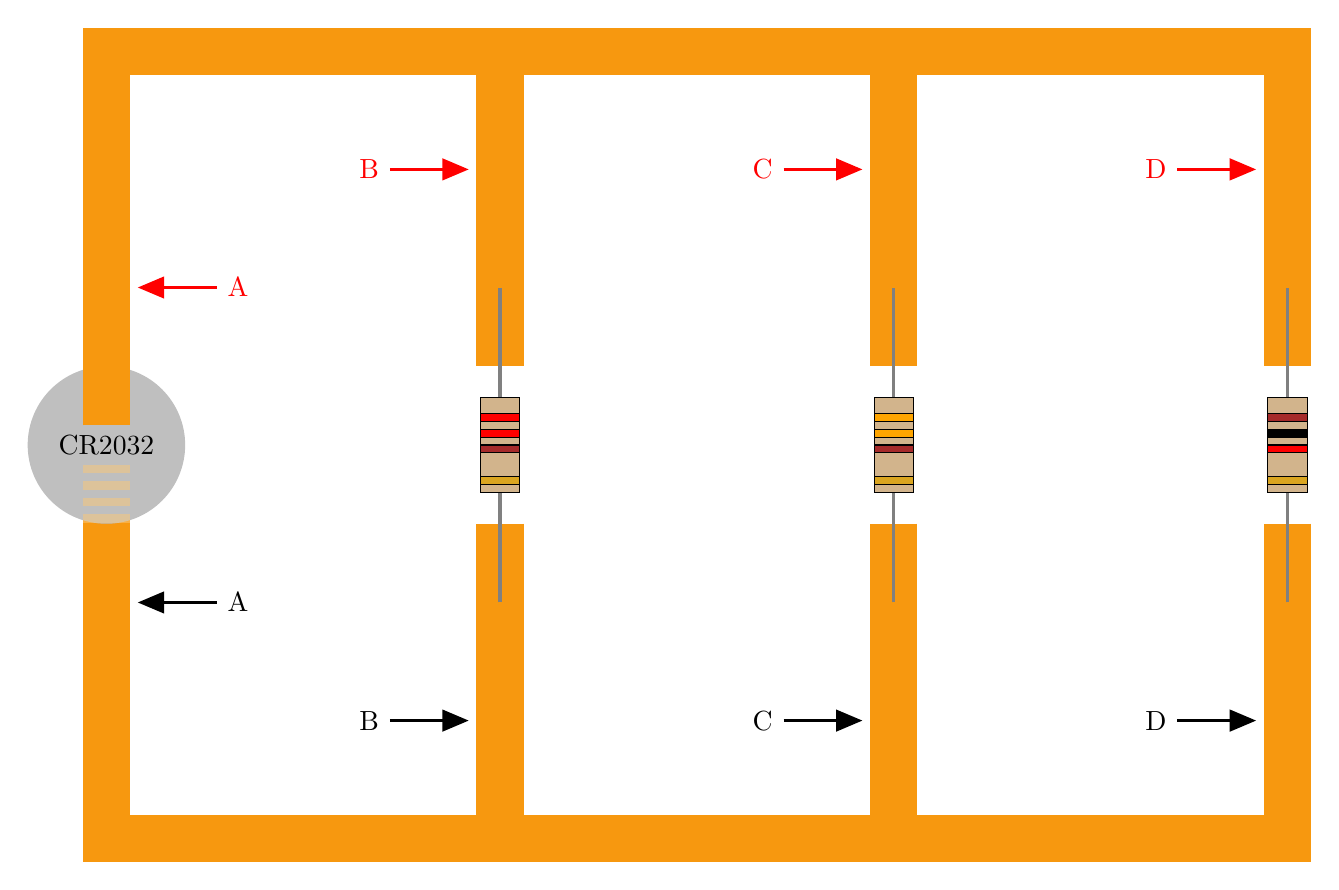
\begin{tikzpicture}
            \draw[line width=6mm,YellowOrange] (0, 0) -- (0, 5) -- (10, 5) -- (10, 1);
            \draw[line width=6mm,YellowOrange] (10, -1) -- (10, -5) -- (0, -5) -- (0, 0);
            \draw[line width=6mm,YellowOrange] (10, 5) -- (15, 5) -- (15, 1);

            \draw[line width=6mm,YellowOrange] (5, 5) -- (5, 1);
            \draw[line width=6mm,YellowOrange] (5, -1) -- (5, -5);
            \draw[line width=6mm,YellowOrange] (15, -1) -- (15, -5) -- (10, -5);

            \fill[black!25] (0, 0) circle (10mm);            
            \draw[line width=6mm, dashed,YellowOrange!50,draw opacity=0.5] (0, -0.25) -- (0, -1);
            \draw[line width=6mm,YellowOrange] (0, 0.25) -- (0, 1);
            \node[align=center] at (0, 0) {CR2032};

            \draw[->,>=triangle 45,very thick,red] (1.4, 2) node[right] {A} -- (0.4, 2);
            \draw[->,>=triangle 45,very thick,black] (1.4, -2) node[right] {A} -- (0.4, -2);

            \draw[->,>=triangle 45,very thick,red] (3.6, 3.5) node[left] {B} --(4.6, 3.5);
            \draw[->,>=triangle 45,very thick,black] (3.6, -3.5) node[left] {B} -- (4.6, -3.5);

            \draw[->,>=triangle 45,very thick,red] (8.6, 3.5) node[left] {C} --(9.6, 3.5);
            \draw[->,>=triangle 45,very thick,black] (8.6, -3.5) node[left] {C} -- (9.6, -3.5);            

            \draw[->,>=triangle 45,very thick,red] (13.6, 3.5) node[left] {D} --(14.6, 3.5);
            \draw[->,>=triangle 45,very thick,black] (13.6, -3.5) node[left] {D} -- (14.6, -3.5);           
            
            \coordinate (R1) at (5, -2);
            %220 Ohms
            \draw[very thick, black!50] (R1) -- ($(R1) + (0, 4)$);
            \draw[fill=Tan] ($(R1) + (0.25, 1.4)$) rectangle ($(R1) + (-0.25, 2.6)$);
            \draw[fill=Red] ($(R1) + (0.25, 2.4)$) rectangle ($(R1) + (-0.25, 2.3)$);
            \draw[fill=Red] ($(R1) + (0.25, 2.2)$) rectangle ($(R1) + (-0.25, 2.1)$);
            \draw[fill=Brown] ($(R1) + (0.25, 2.0)$) rectangle ($(R1) + (-0.25, 1.9)$);
            \draw[fill=Goldenrod] ($(R1) + (0.25, 1.6)$) rectangle ($(R1) + (-0.25, 1.5)$);

            \coordinate (R1) at (10, -2);
            %330 Ohms
            \draw[very thick, black!50] (R1) -- ($(R1) + (0, 4)$);
            \draw[fill=Tan] ($(R1) + (0.25, 1.4)$) rectangle ($(R1) + (-0.25, 2.6)$);
            \draw[fill=Orange] ($(R1) + (0.25, 2.4)$) rectangle ($(R1) + (-0.25, 2.3)$);
            \draw[fill=Orange] ($(R1) + (0.25, 2.2)$) rectangle ($(R1) + (-0.25, 2.1)$);
            \draw[fill=Brown] ($(R1) + (0.25, 2.0)$) rectangle ($(R1) + (-0.25, 1.9)$);
            \draw[fill=Goldenrod] ($(R1) + (0.25, 1.6)$) rectangle ($(R1) + (-0.25, 1.5)$);

            \coordinate (R1) at (15, -2);
            %1k Ohms
            \draw[very thick, black!50] (R1) -- ($(R1) + (0, 4)$);
            \draw[fill=Tan] ($(R1) + (0.25, 1.4)$) rectangle ($(R1) + (-0.25, 2.6)$);
            \draw[fill=Brown] ($(R1) + (0.25, 2.4)$) rectangle ($(R1) + (-0.25, 2.3)$);
            \draw[fill=Black] ($(R1) + (0.25, 2.2)$) rectangle ($(R1) + (-0.25, 2.1)$);
            \draw[fill=Red] ($(R1) + (0.25, 2.0)$) rectangle ($(R1) + (-0.25, 1.9)$);
            \draw[fill=Goldenrod] ($(R1) + (0.25, 1.6)$) rectangle ($(R1) + (-0.25, 1.5)$);
        \end{tikzpicture}
    \end{center}   
    
    \begin{minipage}[t]{0.35\boxwidth}\vspace*{0pt}
        \begin{center}
            \newcolumntype{C}{>{\centering\arraybackslash}X}
            \begin{tabularx}{\boxwidth}{| >{\bfseries\centering\arraybackslash}p{0.2cm} | C | C | C | C |}
                \hline
                \cellcolor{black!25} & \textbf{A} & \textbf{B} & \textbf{C} & \textbf{D}\\\hline
                \raisebox{-0.5cm}{V} & & & & \\[1cm]\hline
                \raisebox{-0.5cm}{R} & & & & \\[1cm]\hline
                \raisebox{-0.5cm}{I} & & & & \\[1cm]\hline
            \end{tabularx}
        \end{center}
    \end{minipage}
    \begin{minipage}{0.02\boxwidth}
        \ 

    \end{minipage}
    \begin{minipage}[t]{0.6\boxwidth}\vspace*{0pt}
        \begin{tabularx}{\boxwidth}{| X |}
            \hline
            \ATLHeader{Communication Skills}\\\hline
            \ATLSkill{...make inferences and draw conclusions...}\\\hline
            \QuestionBox{Using a table or the \emph{total resistance of a parallel circuit} formula, determine what the total resistance in this circuit should be. Explain why this value does not \emph{exactly} match the multimeter measurement for total resistance.}\\\hline
            \ \\[3.5cm]\hline
        \end{tabularx}
    \end{minipage}
    \pagebreak
 
    \begin{tabularx}{\boxwidth}{| X | }
        \hline
        \FormativeHeader \\\hline
        \QuestionBox{Using only three resistors from your kit, what is the closest a parallel circuit can get to $100\ \Omega$ total resistance? What resistors get you that close?}\\\hline
        \ \\[1.5cm]\hline
        \QuestionBox{A \emph{combined} circuit has components placed in series and in parallel. The following circuit diagram is a simple example of a combined circuit.} \\
        \cellcolor{QuestionHeaderBG}\hfill 
        \begin{circuitikz}
            \draw (0, 1) node[left] {+} to [battery1,l_,label=3V] (0, 0);
            \draw (0, 1) |- (1, 2) to [european resistor,label=$220 \Omega$] (2, 2) -| (3, 1.5) -| (2.5, 1) to [european resistor,l_,label=$1\ \text{k}\Omega$] (2.5, 0) |- (3, -0.5);
            \draw (3, 1.5) -| (3.5, 1) to [european resistor,label=$1\ \text{k}\Omega$] (3.5, 0) |- (3, -0.5);
            \draw (3, -0.5) |- (0, -1) -- (0, 0);
        \end{circuitikz}
        \hfill\, \\
        \cellcolor{QuestionHeaderBG}In such a circuit, the parallel resistors can be counted as if they were a single resistor in series with the rest of the circuit, but with a value calculated based on the resistors in parallel formula given in the technical background.\\[1cm]
        \cellcolor{QuestionHeaderBG}Calculate the total resistance in the circuit example given above.\\\hline
        \ \\[1.5cm]\hline
        \QuestionBox{Create a paper circuit below of the above circuit and test your calculation using a multimeter.}\\\hline
        \ \\[12cm]\hline
    \end{tabularx}

    \pagebreak
    \section{Reflections}
    \begin{tabularx}{\boxwidth}{| X |}
        \hline
        \ATLHeader{Communication Skills}\\\hline
        \ATLSkill{...make inferences and draw conclusions...}\\\hline
        \QuestionBox{In what ways does your own understanding of a topic benefit from first making inferences about what is happening before verification through experiment of study?}\\\hline
        \ \\[3.5cm]\hline
        \ATLSkill{...use and interpret a range of discipline-specific terms and symbols...}\\\hline
        \QuestionBox{If you open up any electronic device, it is unlikely that the circuits are arranged as neatly as they are in a circuit diagram or your paper circuits. This is because the paper circuits have a lot of wasted space which makes it difficult to fit into small components or devices with odd-angled surfaces. Despite this, it is very common for circuits to be described in circuit diagrams similiar to the ones you've seen so far. Why do yo think showing components in a diagram different from how they will be physically arranged remains important for analyzing circuits?}\\\hline
        \ \\[3.5cm]\hline
    \end{tabularx}

    \bigskip
    \begin{tabularx}{\boxwidth}{| X |}
        \hline
        \QuestionBox{What aspect of this lesson was the most challenging for you? How did you overcome that challenge?}\\\hline
        \ \\[3.5cm]\hline
        \QuestionBox{Select the option which best reflects how confident you are in applying what you have learend in this lesson.}\\\hline
        \, \hfill \Sadey[5][orange] \hfill \Neutrey[5][gray] \hfill \Smiley[5][cyan] \hfill \,\\\hline
        \QuestionBox{What additional questions do you still have about this lesson's content?}\\\hline
        \ \\[3.5cm]\hline
    \end{tabularx}    
\end{document}